\documentclass[conference]{IEEEtran}
\usepackage[utf8]{inputenc}
\usepackage[T1]{fontenc}
\usepackage[spanish]{babel}
\usepackage{amsmath,amssymb}
\usepackage{graphicx}
\usepackage{booktabs}
\usepackage{cite}
\usepackage{url}

% Carpeta donde van las figuras exportadas de los notebooks
\graphicspath{{./figs/}}

\begin{document}

\title{Detección de imágenes generadas por IA con adaptación de dominio a fotografías de redes sociales}

\author{
\IEEEauthorblockN{Lautaro Valentín Caminoa}
\IEEEauthorblockA{Universidad de San Andrés\\
lcaminoa@udesa.edu.ar}
\and
\IEEEauthorblockN{Francisco Krinisky}
\IEEEauthorblockA{Universidad de San Andrés\\
kfrancisco@udesa.edu.ar}
}

\maketitle

% =====================================================================
\begin{abstract}
La proliferación de generadores de imágenes por difusión hace cada vez más difícil distinguir fotografías reales de imágenes sintéticas, con implicancias directas sobre la desinformación. En este trabajo se comparan cuatro modelos de clasificación binaria (real vs.\ generada por IA) entrenados sobre 60\,000 imágenes de paisajes, naturaleza y arte: un MLP sobre componentes principales (PCA), una CNN entrenada desde cero y ResNet50 preentrenada bajo dos estrategias de transfer learning (feature extraction y fine-tuning). El mejor modelo (fine-tuning) alcanza 93.4\% de accuracy en test, pero su rendimiento cae a 62.5\% sobre fotografías cotidianas de redes sociales por el corrimiento de dominio (domain shift). Como extensión, se aplica un fine-tuning incremental con learning rate muy reducido ($10^{-5}$) sobre el dataset itw-sm (imágenes de Facebook, X, Instagram y LinkedIn), que eleva la accuracy en el dominio nuevo a 94.5\% con una degradación acotada de 7 puntos en el dominio original, cuantificando en la práctica el compromiso entre adaptación y olvido catastrófico.
\end{abstract}

% =====================================================================
\section{Introducción}

Los modelos generativos de imágenes (Stable Diffusion, DALL-E, Midjourney) producen resultados cada vez más fotorrealistas. Esto plantea un problema concreto: verificar si una imagen que circula en internet fue capturada por una cámara o sintetizada por un modelo. La detección automática de imágenes generadas es, por lo tanto, una herramienta relevante para la moderación de contenido y la lucha contra la desinformación.

La entrada de nuestros algoritmos es una imagen RGB redimensionada a $224 \times 224$ píxeles (o $128 \times 128$ para el MLP). Utilizamos cuatro clasificadores —un perceptrón multicapa sobre componentes de PCA, una red convolucional entrenada desde cero, y ResNet50 preentrenada en ImageNet con dos estrategias de transfer learning— para obtener una predicción binaria: \emph{real} o \emph{generada por IA}.

La tarea básica consiste en entrenar y comparar estos cuatro modelos sobre un dataset público de Kaggle. Durante la evaluación cualitativa detectamos una limitación importante: los modelos fallan sistemáticamente sobre fotografías cotidianas (selfies, comida, eventos), ya que las imágenes reales del dataset de entrenamiento son exclusivamente paisajes, naturaleza, arquitectura y arte. Esta observación motivó la \textbf{extensión} del trabajo: un quinto modelo obtenido por fine-tuning incremental sobre imágenes de redes sociales, que estudia empíricamente el problema de adaptación de dominio y el olvido catastrófico asociado.

% =====================================================================
\section{Conjunto de datos y características}

\subsection{Dataset principal}

Se utilizó el dataset \emph{AI-Generated Images vs Real Images} de Kaggle \cite{kaggle-dataset}, con 60\,000 imágenes balanceadas (50\% reales / 50\% generadas). Las imágenes reales son fotografías de paisajes, naturaleza, arquitectura y arte; las generadas son versiones sintéticas producidas por modelos de difusión.

El dataset original provee 48\,000 imágenes de entrenamiento y 12\,000 de prueba. Conservamos las 48\,000 como conjunto de \emph{train} y dividimos las 12\,000 restantes en \emph{validación} y \emph{test} (50/50, estratificado por clase), resultando en una partición 80/10/10. Durante el preprocesamiento se descartaron 12 imágenes corruptas (archivos truncados), quedando 47\,991 / 6\,000 / 5\,997 imágenes; el desbalance resultante es inferior al 0.01\%.

Un hallazgo del análisis exploratorio: las imágenes reales son mayormente rectangulares (resoluciones de cámara y celular, p.\ ej.\ $1080 \times 1620$), mientras que las generadas son mayormente cuadradas ($1024 \times 1024$, $2048 \times 2048$), resoluciones típicas de los generadores. Al redimensionar todo a $224 \times 224$ esta señal espuria se elimina y los modelos deben aprender señales de textura y coherencia.

\begin{figure}[t]
\centering
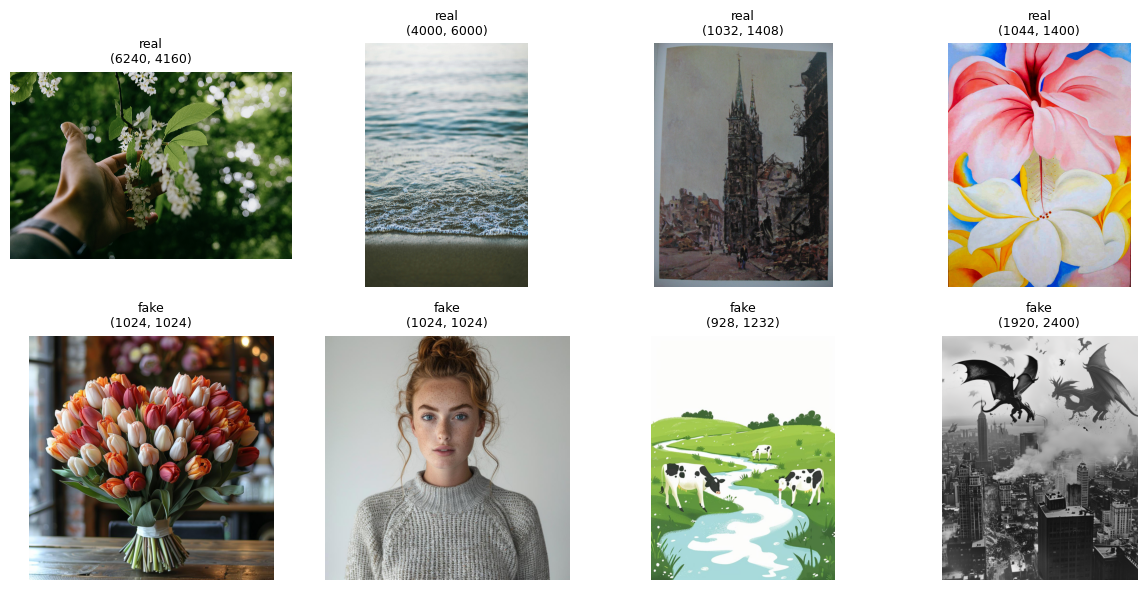
\includegraphics[width=0.88\columnwidth]{fig_muestras_dataset.png}
\caption{Muestras del dataset principal: imágenes reales (fila superior) vs.\ generadas por IA (fila inferior).}
\label{fig:muestras}
\end{figure}

\subsection{Preprocesamiento y aumento de datos}

Todas las imágenes se redimensionaron a $224 \times 224$ px (interpolación de Lanczos), el tamaño de entrada estándar de ResNet50, y se normalizaron con las estadísticas de ImageNet ($\mu = [0.485, 0.456, 0.406]$, $\sigma = [0.229, 0.224, 0.225]$). La normalización se aplicó a los cuatro modelos para que el preprocesamiento fuera idéntico y las comparaciones justas. Sobre el conjunto de train se aplicó aumento de datos liviano: flip horizontal aleatorio, rotación de $\pm 10°$ y variación aleatoria de brillo y contraste.

\subsection{Extracción de características para el MLP}

El MLP no puede operar sobre los $224 \times 224 \times 3 = 150\,528$ píxeles crudos. Las imágenes se cargaron a $128 \times 128 \times 3$ (49\,152 features) y se comprimieron mediante PCA ajustado sobre una muestra aleatoria de 5\,000 imágenes de train. Conservando el 90\% de la varianza se obtuvieron \textbf{321 componentes}. Se usó \texttt{whiten=True} para llevar cada componente a varianza unitaria: sin este paso, la primera componente tiene una escala $\sim$10\,000 veces mayor que las últimas y el gradiente del MLP se desestabiliza. La Fig.~\ref{fig:pca-rec} muestra que la reconstrucción desde 321 componentes preserva la estructura global de la imagen, es decir que la compresión retiene señal suficiente para clasificar.

\begin{figure}[t]
\centering
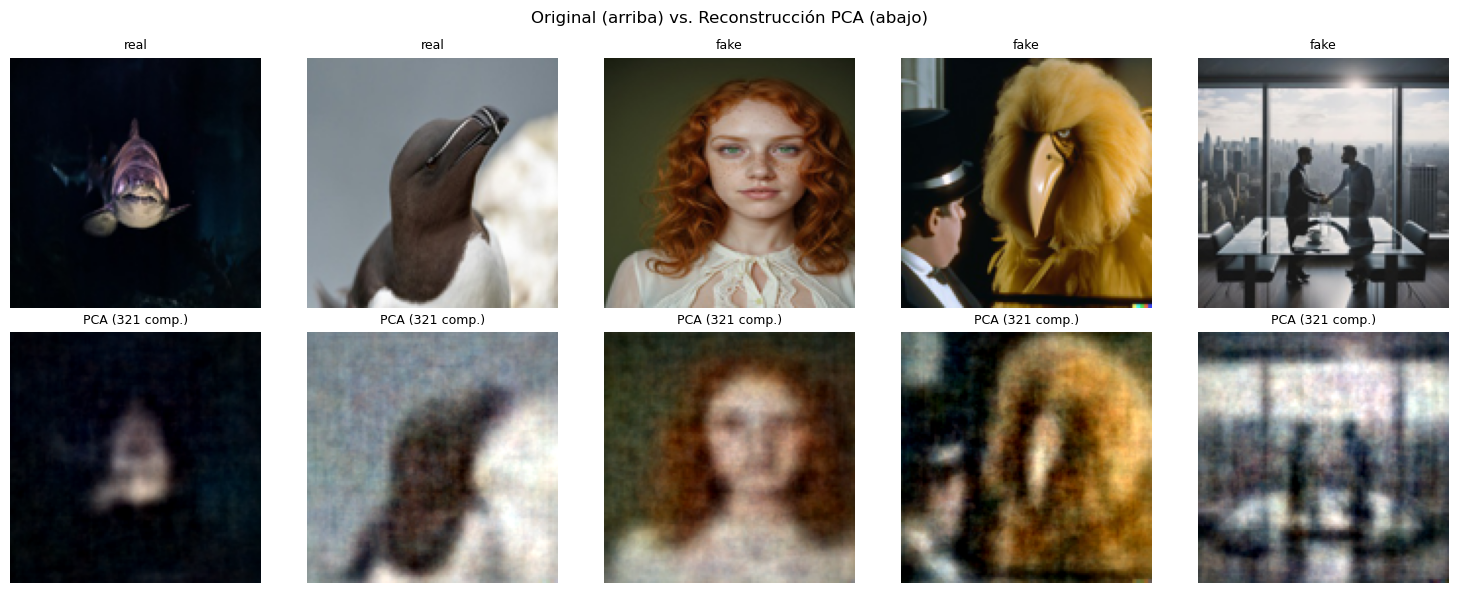
\includegraphics[width=0.9\columnwidth]{fig_pca_reconstruccion.png}
\caption{Imágenes originales (arriba) y sus reconstrucciones desde las 321 componentes de PCA (abajo): la compresión al 90\% de la varianza preserva la estructura global.}
\label{fig:pca-rec}
\end{figure}

\subsection{Dataset de la extensión: itw-sm}

Para la adaptación de dominio se utilizó el dataset \emph{itw-sm} (In The Wild -- Social Media) \cite{itwsm}, de acceso restringido en HuggingFace: 10\,000 imágenes (5\,000 reales / 5\,000 generadas) extraídas de Facebook, X, Instagram y LinkedIn, con contenido cotidiano (Fig.~\ref{fig:itwsm}). Se dividió 80/10/10 estratificado en train/val/test.

\begin{figure*}[t]
\centering
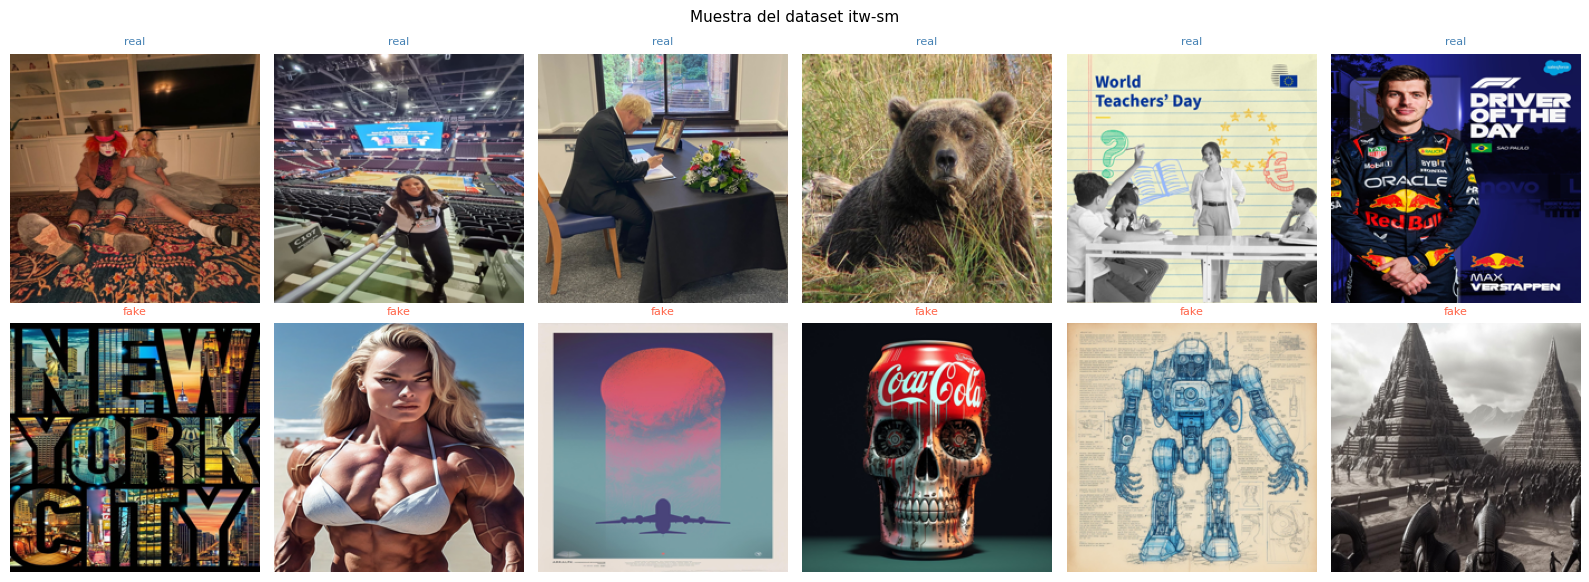
\includegraphics[width=0.46\textwidth]{fig_muestra_itwsm.png}
\caption{Muestras del dataset itw-sm: imágenes reales (fila superior) y generadas por IA (fila inferior) extraídas de redes sociales. El contenido cotidiano contrasta con los paisajes y el arte del dataset principal.}
\label{fig:itwsm}
\end{figure*}

% =====================================================================
\section{Metodología}

Los cuatro modelos son clasificadores binarios entrenados con la misma función de pérdida y el mismo protocolo. La salida de cada red es un logit $z \in \mathbb{R}$ que se convierte en probabilidad mediante la función sigmoidea $\hat{p} = \sigma(z) = (1+e^{-z})^{-1}$, y se clasifica como \emph{generada por IA} si $\hat{p} \geq 0.5$. La pérdida es la entropía cruzada binaria sobre logits (\texttt{BCEWithLogitsLoss}), numéricamente más estable que aplicar sigmoide y BCE por separado:
\begin{equation}
\mathcal{L}(z, y) = -\left[ y \log \sigma(z) + (1-y) \log (1 - \sigma(z)) \right]
\end{equation}
donde $y \in \{0, 1\}$ es la etiqueta (0 = real, 1 = generada).

\subsection{MLP sobre componentes PCA}

Arquitectura $321 \to 512 \to 256 \to 1$ con activaciones ReLU y dropout de 0.4 en las capas ocultas. Actúa como \emph{baseline}: al aplanar la imagen trata cada píxel (proyectado por PCA) como una feature independiente, sin explotar la estructura espacial.

\subsection{CNN entrenada desde cero}

Dado que las redes convolucionales van más allá de lo cubierto en el curso, se describe brevemente su funcionamiento. Una capa convolucional reemplaza el producto matricial denso del MLP por la convolución de la entrada con un banco de filtros pequeños (aquí $3 \times 3$) que se deslizan sobre la imagen. La activación del filtro $k$ en la posición $(i,j)$ es
\begin{equation}
z^{(k)}_{i,j} = b^{(k)} + \sum_{c} \sum_{m,n} w^{(k)}_{c,m,n} \, x_{c,\,i+m,\,j+n}
\end{equation}
donde $c$ recorre los canales de entrada y $(m,n)$ la ventana del filtro. Dos propiedades hacen a las CNN superiores al MLP para imágenes: los \emph{pesos compartidos} (el mismo filtro se aplica en toda la imagen, reduciendo drásticamente los parámetros y detectando un patrón sin importar dónde aparezca) y la \emph{localidad} (cada activación depende solo de una vecindad de píxeles, explotando la estructura espacial que el MLP ignora). Entre capas se intercala \emph{max pooling}, que reduce el mapa espacial a la mitad quedándose con la activación máxima de cada ventana $2 \times 2$, y \emph{batch normalization} \cite{batchnorm}, que normaliza las activaciones para estabilizar el entrenamiento. Al apilar capas, la red construye una jerarquía: las primeras detectan bordes y texturas simples; las profundas, estructuras de alto nivel.

Nuestra arquitectura tiene cuatro bloques convolucionales con filtros crecientes ($32 \to 64 \to 128 \to 256$), cada uno compuesto por Conv $3\times3$ + BatchNorm + ReLU + MaxPool $2\times2$. El mapa final de $14 \times 14 \times 256$ se aplana (50\,176 valores) y pasa por dos capas densas ($512 \to 1$) con dropout de 0.5. Total: 26.1M de parámetros entrenables.

\subsection{Transfer learning con ResNet50}

Se utilizó ResNet50 \cite{resnet} preentrenada en ImageNet \cite{imagenet} bajo dos estrategias:

\begin{itemize}
\item \textbf{Feature extraction (FE):} todo el backbone congelado; solo se entrena la capa de salida ($2048 \to 1$), es decir 2\,049 parámetros.
\item \textbf{Fine-tuning (FT):} se descongela además \texttt{layer4} (el último bloque residual), totalizando $\sim$15M de parámetros entrenables (63.7\%). Las primeras capas detectan features genéricos (bordes, texturas simples) que transfieren bien; \texttt{layer4} captura estructuras de alto nivel específicas del dominio y es la que más se beneficia de adaptarse a la tarea.
\end{itemize}

\subsection{Extensión: fine-tuning incremental (adaptación de dominio)}

Partiendo de los pesos del modelo FT ya entrenado, se continuó el entrenamiento sobre las imágenes de itw-sm descongelando las mismas capas (\texttt{layer4} + fc) pero con un learning rate 100 veces menor ($10^{-5}$). El objetivo del LR reducido es mitigar el \emph{olvido catastrófico} \cite{catastrophic}: que el modelo incorpore el dominio nuevo ajustando sus pesos mínimamente, sin destruir lo aprendido sobre el dominio original.

\subsection{Protocolo de entrenamiento}

Todos los modelos se entrenaron con Adam \cite{adam} (weight decay $10^{-4}$), batch size 128, máximo 50 epochs y \emph{early stopping} con paciencia de 10 epochs sobre la pérdida de validación, guardando el checkpoint de menor \texttt{val\_loss}. La semilla aleatoria se fijó en 26 para reproducibilidad. Para la adaptación de dominio se usó batch size 32, máximo 20 epochs y paciencia 5. Implementación en PyTorch \cite{pytorch} y scikit-learn \cite{sklearn}.

No se realizó validación cruzada: con 48\,000 imágenes de entrenamiento y redes profundas, repetir cada entrenamiento $k$ veces resulta computacionalmente prohibitivo. En su lugar se utilizó un conjunto de validación fijo de 6\,000 imágenes, cuyo tamaño es suficiente para obtener estimaciones estables de las métricas y decidir el early stopping.

% =====================================================================
\section{Experimentos, resultados y discusión}

\subsection{Selección de hiperparámetros}

El learning rate se ajustó por estrategia: $10^{-3}$ (valor por defecto de Adam) para MLP, CNN y FE, donde los pesos entrenados parten de cero; $10^{-4}$ para FT, un orden de magnitud menor para actualizar pesos preentrenados con pasos pequeños sin destruir los features de ImageNet; y $10^{-5}$ para la adaptación incremental, dos órdenes menor, priorizando la preservación del conocimiento previo. El batch size de 128 balancea estabilidad del gradiente y memoria de GPU; en la adaptación se redujo a 32 por la decodificación on-the-fly de las imágenes de HuggingFace. Con early stopping, los modelos frenaron en los epochs 14 (MLP), 43 (CNN), 23 (FE) y 12 (FT); la adaptación completó los 20 epochs.

\subsection{Métricas}

Reportamos accuracy, precision, recall y F1 sobre el test set, con la clase positiva = \emph{generada por IA}:
\begin{equation}
\text{Prec} = \frac{TP}{TP+FP},\;
\text{Rec} = \frac{TP}{TP+FN},\;
F_1 = \frac{2\,\text{Prec}\cdot\text{Rec}}{\text{Prec}+\text{Rec}}
\end{equation}
En este contexto, un falso positivo implica acusar de sintética una foto real, y un falso negativo implica dejar pasar una imagen generada.

\subsection{Resultados en el dominio original}

La Tabla~\ref{tab:resultados} resume los resultados de los cuatro modelos sobre el test set (5\,997 imágenes) y la Fig.~\ref{fig:comparacion} los compara visualmente.

\begin{table}[t]
\caption{Métricas sobre el test set del dominio original}
\label{tab:resultados}
\centering
\begin{tabular}{lcccc}
\toprule
\textbf{Modelo} & \textbf{Accuracy} & \textbf{Precision} & \textbf{Recall} & \textbf{F1} \\
\midrule
MLP + PCA    & 0.7237 & 0.7017 & 0.7787 & 0.7382 \\
CNN          & 0.8843 & 0.9037 & 0.8603 & 0.8815 \\
ResNet50 FE  & 0.8808 & 0.8777 & 0.8850 & 0.8813 \\
ResNet50 FT  & \textbf{0.9335} & \textbf{0.9257} & \textbf{0.9427} & \textbf{0.9341} \\
\bottomrule
\end{tabular}
\end{table}

\begin{figure}[t]
\centering
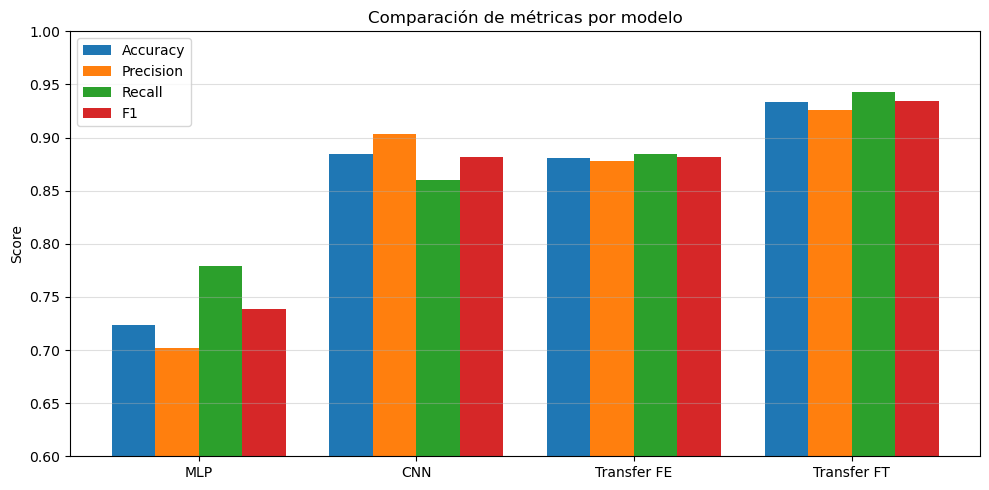
\includegraphics[width=0.92\columnwidth]{fig_comparacion_metricas.png}
\caption{Comparación de métricas por modelo sobre el test set.}
\label{fig:comparacion}
\end{figure}

El MLP (72.4\%) confirma que la estructura espacial es esencial para esta tarea: PCA descarta información que las convoluciones sí explotan. La CNN desde cero y feature extraction empatan ($\sim$88\%), un resultado interesante: los features genéricos de ImageNet, con solo 2\,049 parámetros entrenados, igualan a una red de 26M de parámetros entrenada específicamente para la tarea. El fine-tuning domina (93.4\%): adaptar \texttt{layer4} permite capturar los artefactos de difusión que no existen en ImageNet.

El análisis de la distribución de probabilidades predichas (Fig.~\ref{fig:probs-ft}) refuerza este ordenamiento: el MLP produce predicciones dispersas y poco confiadas (gran masa en el rango 0.3--0.7), mientras que FT es el más polarizado, con el 82\% de las imágenes en los extremos (0.0--0.1 o 0.9--1.0). La matriz de confusión de FT (Fig.~\ref{fig:confusion-ft}) muestra errores balanceados entre ambas clases.

\begin{figure}[t]
\centering
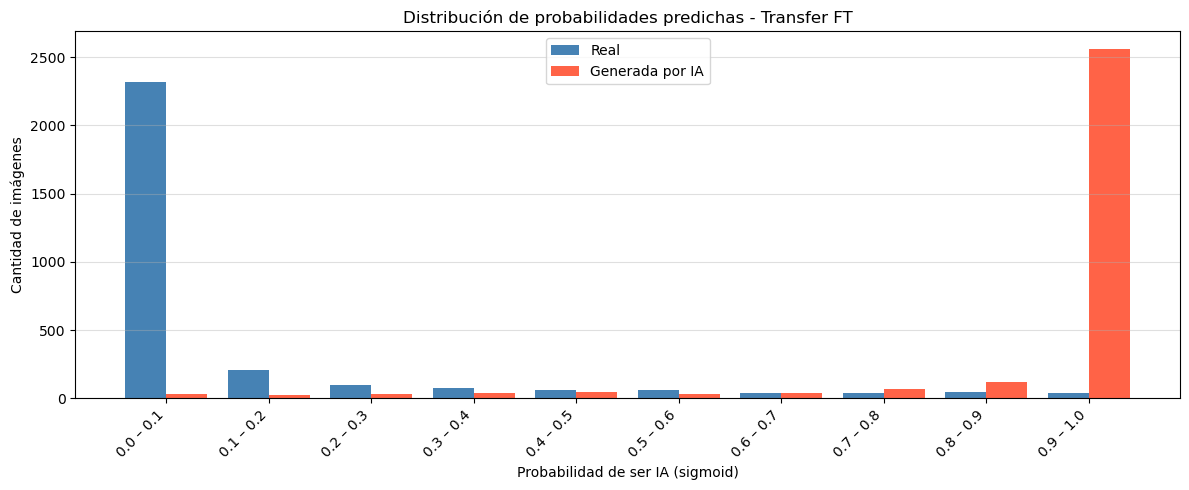
\includegraphics[width=0.92\columnwidth]{fig_distribucion_probs_ft.png}
\caption{Distribución de probabilidades predichas por el modelo FT sobre el test set, separada por clase verdadera.}
\label{fig:probs-ft}
\end{figure}

\begin{figure}[t]
\centering
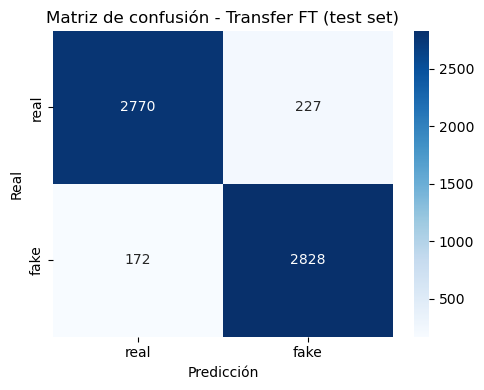
\includegraphics[width=0.62\columnwidth]{fig_matriz_confusion_ft.png}
\caption{Matriz de confusión del modelo FT sobre el test set.}
\label{fig:confusion-ft}
\end{figure}

\subsection{Umbral de clasificación óptimo}

Sobre el conjunto de validación se calculó la curva ROC del modelo FT (Fig.~\ref{fig:roc}, AUC $= 0.9862$) y el umbral que maximiza el índice de Youden $J = TPR - FPR$. El óptimo resultó 0.5965: subir el umbral mejora la precision de 0.9274 a 0.9434 a costa de una leve caída de recall (0.9497 a 0.9390), con mejora marginal de F1 ($+0.003$). Esto confirma que 0.5 ya es una elección razonable para un dataset balanceado.

\begin{figure}[t]
\centering
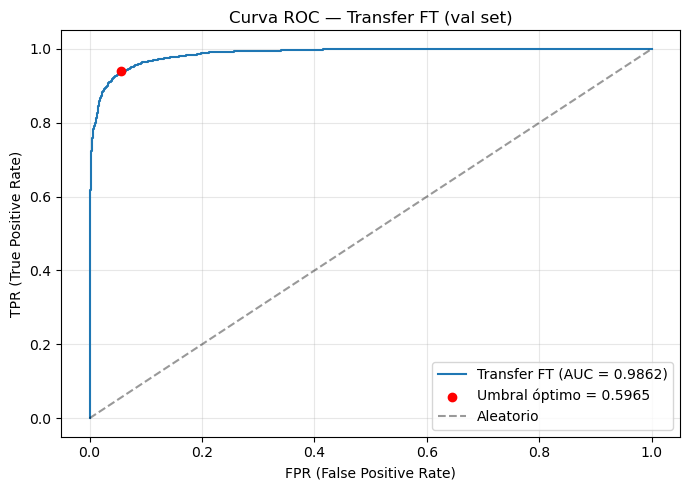
\includegraphics[width=0.72\columnwidth]{fig_roc_ft.png}
\caption{Curva ROC del modelo FT sobre validación, con el umbral óptimo según el índice de Youden.}
\label{fig:roc}
\end{figure}

\subsection{Sobreajuste}

El modelo FT muestra la brecha train/val más pronunciada, esperable con 15M de parámetros: como se observa en la Fig.~\ref{fig:curvas-ft}, la pérdida de train colapsa a 0.016 mientras que la de validación alcanza su mínimo en el epoch 2 (0.149) y luego se estanca en torno a 0.20. Las mitigaciones aplicadas fueron aumento de datos, weight decay, dropout en MLP/CNN y, principalmente, early stopping con checkpoint del mejor epoch de validación: las métricas reportadas corresponden siempre a ese checkpoint y a un test set nunca visto, por lo que la brecha no invalida los resultados. En la adaptación incremental se observó el mismo patrón leve (train 0.037 vs.\ val 0.17 al final) con val\_accuracy estable, señal de sobreajuste incipiente pero no degradante.

\begin{figure}[t]
\centering
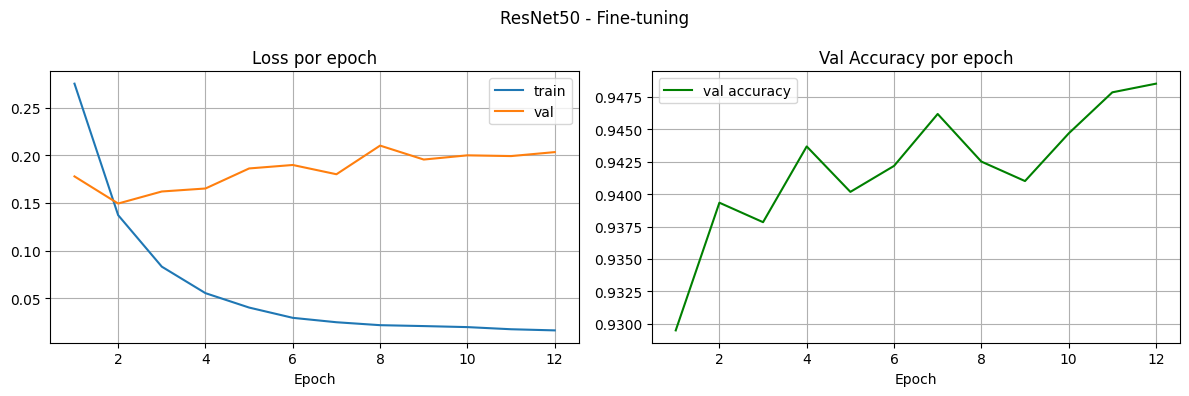
\includegraphics[width=0.95\columnwidth]{fig_curvas_entrenamiento_ft.png}
\caption{Curvas de entrenamiento del fine-tuning de ResNet50: pérdida de train y validación (izquierda) y accuracy de validación (derecha). La divergencia entre curvas de pérdida a partir del epoch 2 evidencia el sobreajuste que el early stopping contiene.}
\label{fig:curvas-ft}
\end{figure}

\subsection{Análisis cualitativo de errores y domain shift}

La Fig.~\ref{fig:errores} muestra imágenes mal clasificadas por la CNN: predominan escenas con texturas suaves o iluminación atípica, donde las señales de síntesis son sutiles.

\begin{figure*}[t]
\centering
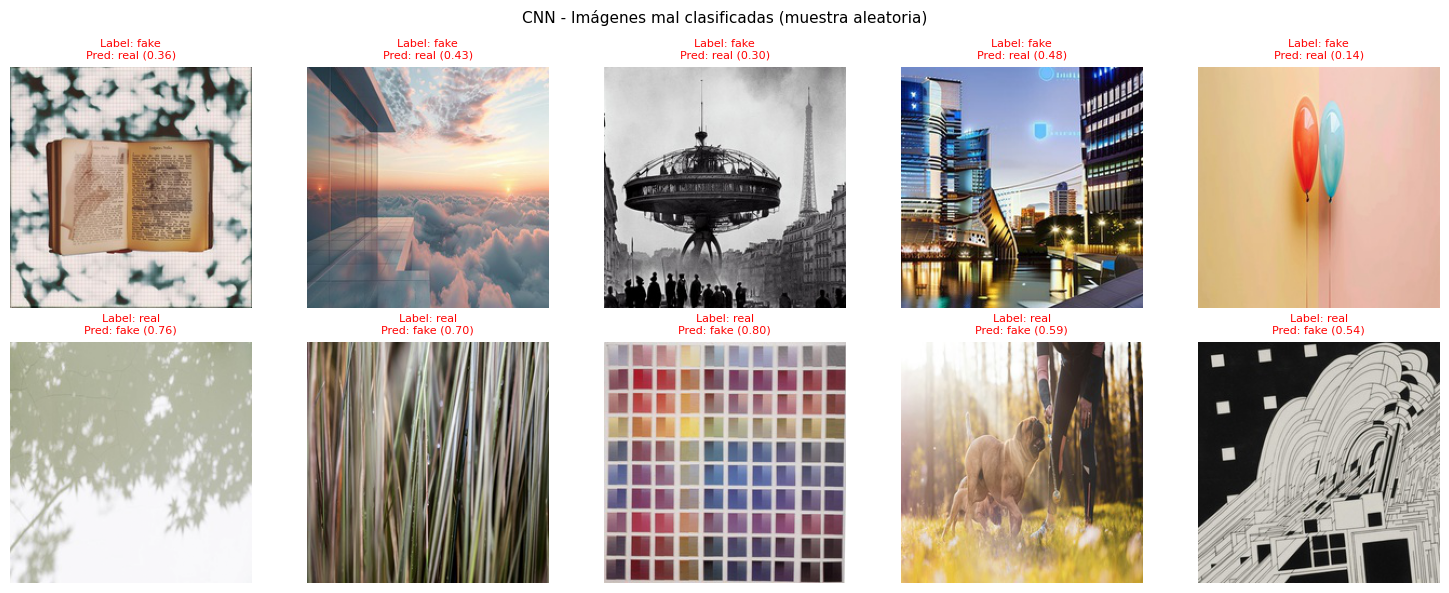
\includegraphics[width=0.48\textwidth]{fig_errores_cnn.png}
\caption{Ejemplos de imágenes del test set mal clasificadas por la CNN, con etiqueta verdadera y probabilidad predicha.}
\label{fig:errores}
\end{figure*}

El hallazgo cualitativo más importante surgió al evaluar los modelos fuera de la distribución: una selfie real es clasificada como generada por IA por la CNN y ambos modelos de transfer learning (Fig.~\ref{fig:selfie}). La explicación es estructural: las imágenes ``reales'' del training set nunca incluyen retratos, por lo que el modelo no aprendió el concepto general de ``foto tomada por un humano'' sino a separar las imágenes del dataset de sus versiones regeneradas.

\begin{figure*}[t]
\centering
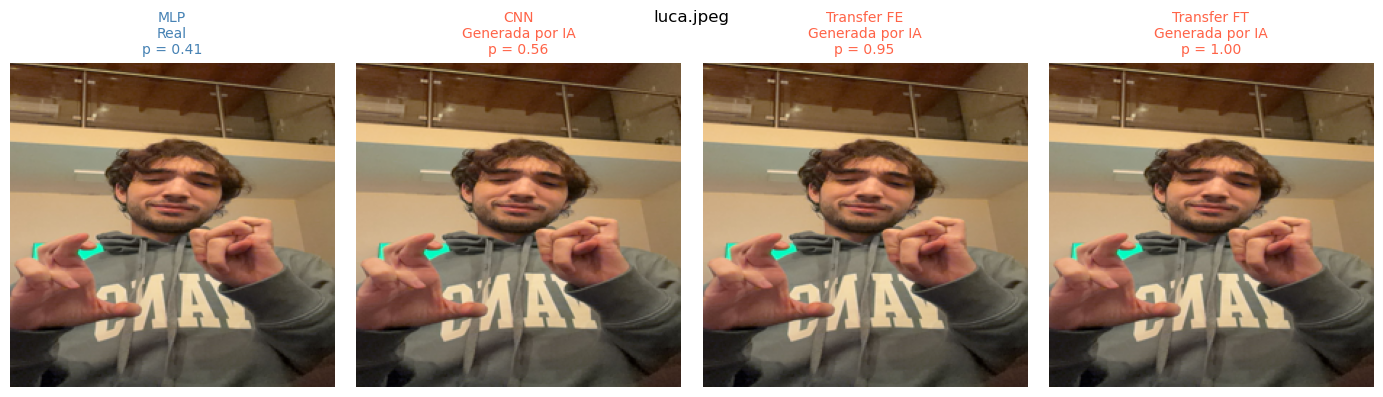
\includegraphics[width=0.48\textwidth]{fig_prediccion_selfie.png}
\caption{Fotografía real de una persona evaluada por los cuatro modelos: tres de ellos la clasifican erróneamente como generada por IA, evidenciando el domain shift.}
\label{fig:selfie}
\end{figure*}

\subsection{Extensión: adaptación de dominio}

La evaluación cuantitativa sobre el test set de itw-sm confirma el problema y descarta que sea una debilidad de alguna arquitectura en particular: los cuatro modelos base rinden cerca del azar (MLP 56.5\%, CNN 64.4\%, FE 60.7\%, FT 62.5\%), con recalls de 0.82--0.97 y precisions de $\sim$0.55--0.59, es decir que clasifican como sintética casi cualquier foto cotidiana real. La limitación es del dominio de entrenamiento, no de los modelos. Tras el fine-tuning incremental (curvas en la Fig.~\ref{fig:adaptacion}), el modelo adaptado se evaluó sobre ambos dominios (Tabla~\ref{tab:adaptacion}).

\begin{table}[t]
\caption{Efecto de la adaptación de dominio (accuracy / F1)}
\label{tab:adaptacion}
\centering
\begin{tabular}{lcc}
\toprule
\textbf{Test set} & \textbf{FT original} & \textbf{FT adaptado} \\
\midrule
Dominio original & \textbf{0.9373} / \textbf{0.9374} & 0.8669 / 0.8733 \\
itw-sm (redes sociales) & 0.6250 / 0.7220 & \textbf{0.9450} / \textbf{0.9453} \\
\bottomrule
\end{tabular}
\end{table}

\begin{figure}[t]
\centering
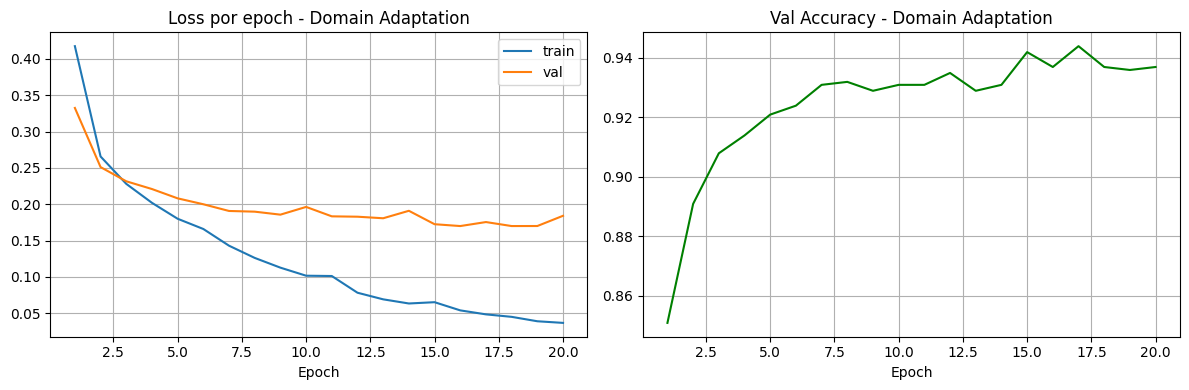
\includegraphics[width=0.95\columnwidth]{fig_curvas_adaptacion.png}
\caption{Curvas del fine-tuning incremental sobre itw-sm: pérdida de train y validación (izquierda) y accuracy de validación (derecha).}
\label{fig:adaptacion}
\end{figure}

La adaptación gana 32 puntos de accuracy en el dominio nuevo (62.5\% $\to$ 94.5\%) a cambio de una caída de 7 puntos en el dominio original (93.7\% $\to$ 86.7\%). La caída confirma la presencia de olvido catastrófico, pero acotada: el learning rate de $10^{-5}$ cumplió su función de preservar la mayor parte del conocimiento previo. El resultado neto es un modelo útil en ambos dominios, y el experimento cuantifica de forma directa el trade-off adaptación/olvido que la literatura describe cualitativamente.

Como validación adicional en condiciones reales, el modelo adaptado se desplegó en una demo web interactiva\footnote{\url{https://panchokrinisky.github.io/web-ai-image-detection/}} donde cualquier usuario puede subir una imagen y obtener la predicción. El código fuente completo del proyecto (notebooks, módulos de entrenamiento y pesos de los cinco modelos) está disponible públicamente\footnote{\url{https://github.com/lcaminoa/ai-image-detection}}.

% =====================================================================
\section{Conclusión y trabajo futuro}

Se compararon cuatro clasificadores de imágenes reales vs.\ generadas por IA sobre un mismo protocolo experimental. El fine-tuning de ResNet50 resultó el mejor modelo (93.4\% accuracy, F1 0.934): los features preentrenados en ImageNet aportan una base que una CNN entrenada desde cero con 48\,000 imágenes no alcanza a superar, y adaptar el último bloque residual permite capturar los artefactos específicos de los generadores. El aporte central del trabajo es la extensión de adaptación de dominio: demostramos que un detector con excelentes métricas in-distribution puede ser inutilizable ante un corrimiento de dominio realista (62.5\% en fotos de redes sociales), y que un fine-tuning incremental con learning rate reducido recupera el rendimiento (94.5\%) con un costo acotado de olvido catastrófico ($-7$ puntos en el dominio original).

Con más tiempo y recursos exploraríamos: (i) \emph{rehearsal} durante la adaptación —mezclar un porcentaje de imágenes del dominio original en el fine-tuning incremental— para reducir el olvido; (ii) arquitecturas más recientes (ViT, ConvNeXt) y detectores basados en frecuencia, más robustos a los artefactos de difusión; y (iii) evaluar la robustez ante degradaciones típicas de redes sociales (recompresión JPEG, reescalado), que alteran las señales de síntesis.

% =====================================================================
\begin{thebibliography}{9}

\bibitem{kaggle-dataset}
T. Zhang, ``AI Generated Images vs Real Images,'' Kaggle, 2024. [En línea]. Disponible: \url{https://www.kaggle.com/datasets/tristanzhang32/ai-generated-images-vs-real-images}

\bibitem{itwsm}
D. Karageorgiou et al., ``itw-sm: In The Wild -- Social Media dataset,'' HuggingFace, 2024. [En línea]. Disponible: \url{https://huggingface.co/datasets/dkarageo/itw-sm}

\bibitem{resnet}
K. He, X. Zhang, S. Ren y J. Sun, ``Deep Residual Learning for Image Recognition,'' en \emph{Proc. IEEE CVPR}, 2016, pp. 770--778.

\bibitem{imagenet}
J. Deng, W. Dong, R. Socher, L.-J. Li, K. Li y L. Fei-Fei, ``ImageNet: A Large-Scale Hierarchical Image Database,'' en \emph{Proc. IEEE CVPR}, 2009, pp. 248--255.

\bibitem{catastrophic}
M. McCloskey y N. J. Cohen, ``Catastrophic Interference in Connectionist Networks: The Sequential Learning Problem,'' \emph{Psychology of Learning and Motivation}, vol. 24, pp. 109--165, 1989.

\bibitem{batchnorm}
S. Ioffe y C. Szegedy, ``Batch Normalization: Accelerating Deep Network Training by Reducing Internal Covariate Shift,'' en \emph{Proc. ICML}, 2015, pp. 448--456.

\bibitem{adam}
D. P. Kingma y J. Ba, ``Adam: A Method for Stochastic Optimization,'' en \emph{Proc. ICLR}, 2015.

\bibitem{pytorch}
A. Paszke et al., ``PyTorch: An Imperative Style, High-Performance Deep Learning Library,'' en \emph{Advances in Neural Information Processing Systems 32}, 2019, pp. 8024--8035.

\bibitem{sklearn}
F. Pedregosa et al., ``Scikit-learn: Machine Learning in Python,'' \emph{Journal of Machine Learning Research}, vol. 12, pp. 2825--2830, 2011.

\end{thebibliography}

\end{document}
